\chapter{Spectral Clustering} \label{chap:spectral}

We provide a summary of traditional random-walk spectral clustering and show how it applies to motif-based clustering.
This chapter mostly follows the relevant sections in the tutorial by U.~Von~Luxburg~\cite{von2007tutorial}, which provides further explanations and proofs.
In Section~\ref{sec:spectral_overview} we give an overview of the spectral clustering procedure.
In Section~\ref{sec:spectral_laplacians} we define the random-walk Laplacian and state some of its useful properties (Proposition~\ref{prop:laplacian}).
In Section~\ref{sec:spectral_graph_cut} we introduce normalised cut (Ncut) as an objective function for graph partitioning.
In Section~\ref{sec:spectral_cluster_extraction} we explore methods of extracting clusters from $\bb{R}^l$-valued embeddings, and in Section~\ref{sec:spectral_algs} we present the algorithms for both traditional and motif-based random-walk spectral clustering.











\section{Overview of spectral clustering} \label{sec:spectral_overview}

Suppose $x_1, \ldots, x_n$ are data points with some associated symmetric similarity matrix $M$ with ${M_{ij} = \mathrm{similarity}(x_i,x_j)}$.
The intuitive aim of clustering is to find a partition $\ca{P}_1, \ldots, \ca{P}_k$ of $\{ x_1, \ldots, x_n \}$ which places similar points in the same group and dissimilar points in different groups.
Where other methods such as $k$-means++  \cite{arthur2007k} and GMM clustering \cite{duda1973pattern} demand some further structure on $x_i$ (such as taking values in $\bb{R}^l$), spectral clustering has no such requirements.

In the context of \emph{undirected} graph clustering, the data points are the vertices of the graph, and a similarity matrix is provided by the graph's adjacency matrix $G$.
To cluster directed graphs, the adjacency matrix must first be symmetrised, traditionally by the transformation $M = G + G^\top$ \cite{Meila2007ClusteringBW}.
This symmetrisation ignores information about edge direction and higher-order structures; and can lead to poor performance, as will be seen in Section~\ref{sec:motif_asymm_dsbms}.

Spectral clustering consists of two steps. Firstly, eigendecomposition of a Laplacian matrix embeds the vertices into $\bb{R}^{l}$. The $k$ clusters are then extracted from this space.










\section{Graph Laplacians} \label{sec:spectral_laplacians}

The Laplacians of an undirected graph are a family of matrices which play a central r\^ole in spectral clustering. While many different graph Laplacians are available, we focus in this dissertation on just the \emph{random-walk Laplacian}, for reasons concerning objective functions, consistency and computation \cite{von2007tutorial, luxburg2004convergence}.


\begin{definition}
Let $\ca{G}$ be an undirected graph with (symmetric) adjacency matrix $G$. The \emph{random-walk Laplacian matrix} of $\ca{G}$ is
$$ L_\mathrm{rw} \vcentcolon= I - D^{-1} G $$
where $I$ is the identity and $D_{ii} \vcentcolon= \sum_j G_{ij}$ is the diagonal matrix of weighted degrees.
\end{definition}


\begin{remark}
$D^{-1} G$ is the transition matrix of a random walk on the vertex set $\ca{V}$ where the probability of the transition $v_i \to v_j$ is proportional to $G_{ij}$.
\end{remark}


\begin{proposition}[Properties of the random-walk Laplacian] \label{prop:laplacian}
$L_\mathrm{rw}$ is positive semi-definite with eigenvalues $0 = \lambda_1 \leq \cdots \leq \lambda_n$.
The multiplicity $k$ of the eigenvalue $0$ is equal to the number of connected components $\ca{P}_1, \ldots, \ca{P}_k$ of $\ca{G}$.
The eigenspace of the eigenvalue $0$ is spanned by the indicator vectors on these components; $ \bb{I}_{\ca{P}_1}, \ldots, \bb{I}_{\ca{P}_k} $.
\end{proposition}

\begin{proof}
See \cite{von2007tutorial}.
\end{proof}









\section{Graph cuts} \label{sec:spectral_graph_cut}

Graph cuts provide objective functions which we seek to minimise while clustering the vertices of a graph.
We look at the normalised cut and its relationship with the random-walk Laplacian.

\begin{definition}
Let $\ca{G}$ be a graph. Let $ \ca{P}_1, \ldots, \ca{P}_k $ be a partition of $\ca{V}$. Then the \emph{normalised cut} \cite{shi2000normalized} of $\ca{G}$ with respect to $ \ca{P}_1, \ldots, \ca{P}_k $ is
%
$$ \mathrm{Ncut}_\ca{G}(\ca{P}_1, \ldots, \ca{P}_k) \vcentcolon= \frac{1}{2} \sum_{i=1}^k \frac{ \mathrm{cut}(\ca{P}_i,\bar{\ca{P}_i}) }{ \mathrm{vol}(\ca{P}_i) } $$
%
where $ \mathrm{cut}(\ca{P}_i,\bar{\ca{P}_i}) \vcentcolon= \sum_{u \in \ca{P}_i, \, v \in \ca{V} \setminus \ca{P}_i} G_{uv}$ and $\mathrm{vol}(\ca{P}_i) \vcentcolon= \sum_{u \in \ca{P}_i} D_{uu}$.

\end{definition}


\begin{remark}
More desirable partitions have a lower Ncut value; the numerators penalise partitions which cut a large number of heavily weighted edges, and the denominators penalise partitions which have highly imbalanced cluster sizes.
\end{remark}


It can be shown \cite{von2007tutorial} that minimising Ncut over partitions $ \ca{P}_1, \ldots, \ca{P}_k $ is equivalent to finding the cluster indicator matrix $H \in \bb{R}^{n \times k}$ minimising
$$ \mathrm{Tr} \big( H^\top (D-G) H \big) $$
subject to
$$ H_{ij} = \mathrm{vol}(\ca{P}_j)^{-\frac{1}{2}} \ \bb{I} \{ v_i \in \ca{P}_j \}\,, \qquad (\dagger) $$
$$ H^\top D H = I\,. $$


Solving this problem is in general \textsf{NP}-hard \cite{wagner1993between}.
However, by dropping the constraint~$(\dagger)$ and applying the Rayleigh Principle \cite{lutkepohl1996handbook}, we find that the solution to this relaxed problem is that $H$ contains the first $k$ eigenvectors of $L_\mathrm{rw}$ as columns \cite{von2007tutorial}.
In practice, to find $k$ clusters it is often sufficient to use only the first $l < k$ eigenvectors of $L_\mathrm{rw}$.








\section{Cluster extraction} \label{sec:spectral_cluster_extraction}

Once Laplacian eigendecomposition has been used to embed the data into $\bb{R}^l$, the clusters may be extracted using a variety of methods. We propose $k$-means++ and eigenvector sweep as two appropriate techniques.


\subsection{\texorpdfstring{$k$}{k}-means++}

$k$-means++ \cite{arthur2007k} is a popular clustering algorithm for data in $\bb{R}^l$.
It aims to minimise the within-cluster sum of squares, based on the standard Euclidean metric on $\bb{R}^l$.
This makes it a reasonable candidate for clustering spectral data, since the Euclidean metric corresponds to notions of `diffusion distance' in the original graph \cite{nadler2006diffusion}.


\subsection{Eigenvector sweep} \label{sec:spectral_sweep}

Eigenvector sweep (Algorithm~\ref{alg:eigenvector_sweep})~\cite{shi2000normalized} offers a more principled technique for cluster extraction when $k=2$ clusters are required, and a single eigenvector (usually the second eigenvector of $L_\mathrm{rw}$) is available. It works by sorting the eigenvector and selecting a splitting point to minimise the Ncut score of the partition generated.

\pagebreak

\begin{algorithm}[H]
\caption{Eigenvector sweep}
\label{alg:eigenvector_sweep}
	
	\SetKwFunction{Main}{EigenvectorSweep}				% name of function
	\newcommand{\MainArgs}{$\ca{G}, x$}		% args to function
		
 	\BlankLine
	\Input{Graph $\ca{G}$, eigenvector $x$}
	\Output{Partition $\ca{P}_1, \ca{P}_2$}
	\BlankLine
	\Function{\Main{\MainArgs}}{
	
		$\hat{x} \leftarrow \mathtt{sort}(x)$ \;
		$\mathrm{Score_{best}} \leftarrow \infty$ \;	
		
		\For{$i$ \In $1, \ldots, n-1$}{
			$\ca{P} \leftarrow \{ \hat{x}_1, \ldots \hat{x}_i \}$ \;
			$\mathrm{Score} \leftarrow \mathrm{Ncut}_\ca{G} (\ca{P}, \ca{V} \setminus \ca{P})$ \;
			\If{$\mathrm{Score} < \mathrm{Score_{best}}$}{
				$\ca{P}_\mathrm{best} \leftarrow \ca{P}$ \;
				$\mathrm{Score_{best}} \leftarrow \mathrm{Score}$ \;
			}
		}
		
		$\ca{P}_1 \leftarrow \ca{P}_\mathrm{best}$ \;		
		$\ca{P}_2 \leftarrow \ca{V} \setminus \ca{P}_\mathrm{best}$ \;		
		
	\Return $\ca{P}_1, \ca{P}_2$
	}
\end{algorithm}
\vspace*{0.5cm}


Figure~\ref{fig:eigenvector_sweep_network} shows a small network with vertices labelled by position in the sorted second eigenvector $\hat{x}$ of $L_\mathrm{rw}$. Figure~\ref{fig:eigenvector_sweep_profile} shows the `sweep profile' of Ncut scores, which is minimised at the splitting point $i=5$. Hence eigenvector sweep chooses the final partition $\ca{P}_1 = \{1, \ldots,5\}, \ \ca{P}_2 = \{6, \ldots,10\}$; as indicated by the vertex colours and dashed line in Figure~\ref{fig:eigenvector_sweep_network}.
%
%
\begin{figure}[H]
	\begin{subfigure}{.49\textwidth}
		\centering
		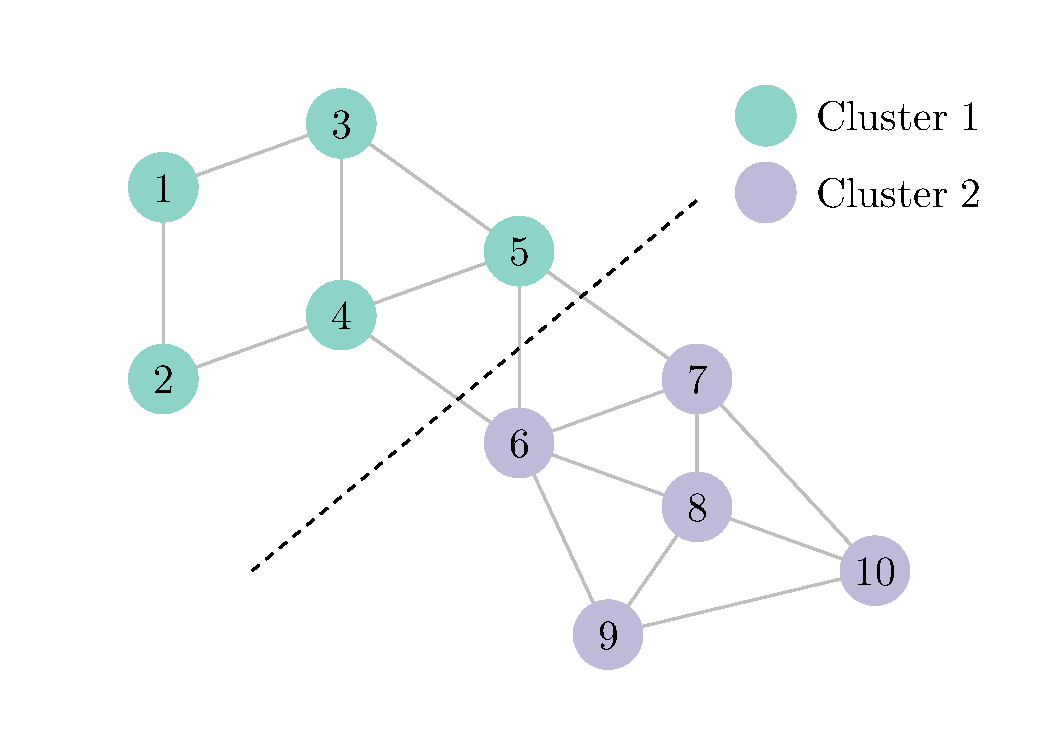
\includegraphics[scale=0.4,draft=false]{../tikz/eigenvector_sweep_network/eigenvector_sweep_network.pdf}
		\caption{A small network}
		\label{fig:eigenvector_sweep_network}
	\end{subfigure}
	%
	\begin{subfigure}{.49\textwidth}
		\centering
		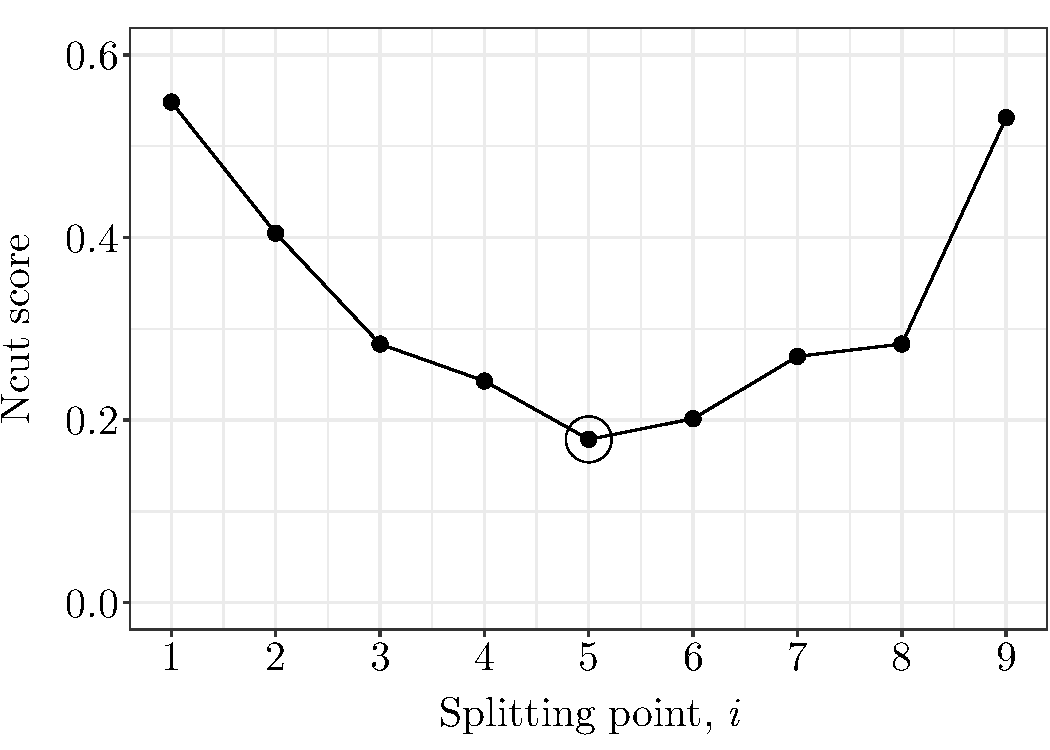
\includegraphics[scale=0.4,draft=false]{../../results/eigenvector_sweep/eigenvector_sweep_scores.pdf}
		\caption{Sweep profile of the network}
		\label{fig:eigenvector_sweep_profile}
	\end{subfigure}
	\caption{Eigenvector sweep selects a partition by minimising Ncut}
	\label{fig:eigenvector_sweep}
\end{figure}
%




\subsection{Cluster evaluation}

When a graph has been clustered, we assign a score to the partition. If the ground-truth clustering is available, we can compare it to our clustering using the \emph{adjusted Rand index} (ARI) \cite{hubert1985comparing}. The ARI between two clusterings has expected value $0$ under random cluster assignment, and maximum value $1$ denoting perfect agreement between the clusterings. A larger ARI indicates a more similar clustering.

If the ground-truth clustering is not available, we can use the objective function Ncut. Clusterings with lower Ncut values partition the graph more agreeably.







\section{Spectral clustering algorithms} \label{sec:spectral_algs}

We present the full random-walk spectral clustering algorithm and show how it can be applied to motif-based random-walk spectral clustering.



\subsection{Random-walk spectral clustering}

Algorithm~\ref{alg:rwspectclust} gives random-walk spectral clustering \cite{von2007tutorial}, which takes a symmetric connected adjacency matrix as input. We use $k$-means++ rather than eigenvector sweep as the cluster extraction method, due to its superior flexibility and computational speed. We drop the first column of $H$ (the first eigenvector of $L_\mathrm{rw}$) since although it should be constant and uninformative (Proposition~\ref{prop:laplacian}), numerical imprecision may give unwanted artefacts. It is worth noting that although the relaxation used in Section~\ref{sec:spectral_graph_cut} is reasonable and often leads to good approximate solutions of the Ncut problem, there are cases where it performs poorly~\cite{guattery1998quality}. The Cheeger inequality~\cite{chung2005laplacians} gives a bound on the error introduced by this relaxation.


\vspace*{0.5cm}
\begin{algorithm}[H]
\caption{Random-walk spectral clustering}
\label{alg:rwspectclust}
	
	\SetKwFunction{Main}{RWSpectClust}				% name of function
	\newcommand{\MainArgs}{$G,k,l$}		% args to function
		
 	\BlankLine
	\Input{Symmetric adjacency matrix $G$, number of clusters $k$, dimension $l$}
	\Output{Partition $\ca{P}_1, \ldots, \ca{P}_k$}
	\BlankLine
	
	\Function{\Main{\MainArgs}}{
		Construct the weighted degree matrix $D_{ii} \leftarrow \sum_j G_{ij}$ \\
		Construct the random walk Laplacian matrix $L_\mathrm{rw} \leftarrow I-D^{-1}G$ \\
		Let $H$ have the first $l$ eigenvectors of $L_\mathrm{rw}$ as columns \\
		Drop the first column of $H$ \\
		Run $k$-means++ on the rows of $H$ with $k$ clusters to produce $\ca{P}_1, \ldots, \ca{P}_k$ \\
	\Return	$\ca{P}_1, \ldots, \ca{P}_k$
	}

\end{algorithm}


\subsection{Motif-based random-walk spectral clustering} \label{sec:spectral_motifrwspectclust}

Algorithm~\ref{alg:motifrwspectclust} gives motif-based random-walk spectral clustering.
Note that although $\ca{G}$ may be a connected graph, there is no guarantee that the MAM is connected too.
Hence $M$ is restricted to its largest connected component $C$ before spectral clustering is applied.
While this may initially seem to be a flaw with motif-based spectral clustering (since not all vertices are assigned to a cluster), in fact it can be very useful; restriction of $M$ can remove vertices which are in some sense not `well connected' to the rest of the graph, which means that only a `core' set of vertices are clustered.
This can result in Algorithm~\ref{alg:motifrwspectclust} making fewer misclassifications with motif-based methods than with traditional spectral clustering, as seen in Section~\ref{sec:motif_polblogs}.

There is ambiguity in whether to use functional or structural MAMs.
While the authors in~\cite{benson2016higher} opt for structural MAMs, we propose to use functional MAMs, for a few reasons.
Firstly, note that $ 0 \leq M^\mathrm{struc}_{ij} \leq M^\mathrm{func}_{ij}$ for all $i,j \in \ca{V}$.
This implies that the largest connected component of $M^\mathrm{func}$ is always at least as large as that of $M^\mathrm{struc}$, meaning that often more vertices can be assigned to a cluster.
Secondly, we argue that functional instances are of more interest than structural motifs, since they specify only `existence' rather than `non-existence' of edges.
For consistency we will therefore use functional MAMs throughout our experiments.

The most computationally expensive part of Algorithm~\ref{alg:motifrwspectclust} is the calculation of the MAM using a formula from Table~\ref{tab:motif_adj_mat_table}. We found this to be feasible for graphs with up to around $n \approx 10 \, 000$ vertices. General notes on hardware and software are given in Section~\ref{sec:notes_hardware}, and timings for MAM computation across a range of graph sizes and sparsities are available in Section~\ref{sec:notes_timing}.




\vspace*{0.5cm}
\begin{algorithm}[H]
\caption{Motif-based random-walk spectral clustering}
\label{alg:motifrwspectclust}
	
	\SetKwFunction{Main}{MotifRWSpectClust}				% name of function
	\newcommand{\MainArgs}{$\ca{G},\mathcal{M},k,l$}		% args to function
		
 	\BlankLine
	\Input{Graph $\ca{G}$, motif $\ca{M}$, number of clusters $k$, dimension $l$}
	\Output{Partition $\ca{P}_1, \ldots, \ca{P}_k$}
	\BlankLine
	
	\Function{\Main{\MainArgs}}{
		Construct the motif adjacency matrix $M$ of the graph $\ca{G}$ with  motif $\ca{M}$ \\
		Let $\tilde{M}$ be $M$ restricted to its largest connected component, $C$ \\
		$\ca{P}_1, \ldots, \ca{P}_k \leftarrow$ \texttt{RWSpectClust($\tilde{M},k,l$)} \\
	\Return	$\ca{P}_1, \ldots, \ca{P}_k$
	}

\end{algorithm}






